% % % % % % % % % % % % % % % % % % % % % % % % % % % % % % % % % % % % % % % % % % % %
%                                                                                     %
% Short Sectioned Assignment LaTeX Template Version 1.0 (5/5/12)                      %
% This template has been downloaded from: http://www.LaTeXTemplates.com               %
%                                                                                     %
% Original author:  Frits Wenneker (http://www.howtotex.com)                          %
%                                                                                     %
% Modified by: Fco Javier Sueza Rodríguez (fcosueza@disroot.org)                      %
%                                                                                     %
% Changes:                                                                            %
%	    - Custom Chapters, Sections and Subsections (titlesec package)                %
%           - Document type scrbook (oneside)                                         %
%           - Use babel-lang-spanish package and marvosym                             %
%           - Use hyperref, enumitem, tcolorbox and glossaries packages               %
%           - Use Time New Roman (mathptmx), Helvetic and Courier fonts               %
%                                                                                     %
% License: CC BY-NC-SA 3.0 (http://creativecommons.org/licenses/by-nc-sa/3.0/)        %
%                                                                                     %
% % % % % % % % % % % % % % % % % % % % % % % % % % % % % % % % % % % % % % % % % % % %

%-----------------------------------------------%
%	              Packages                  %
%-----------------------------------------------%

\documentclass[paper=a4, fontsize=11pt, oneside]{scrbook}

% ---- Text Input/Output ----- %

\usepackage[T1]{fontenc}
\usepackage[utf8]{inputenc}
\usepackage{mathptmx}
\usepackage[scaled=.92]{helvet}
\usepackage{courier}
\usepackage[indent=12pt]{parskip}

\usepackage{geometry}
\geometry{verbose,tmargin=3cm,bmargin=3cm,lmargin=2.6cm,rmargin=2.6cm}

% ---- Language ----- %

\usepackage[spanish]{babel}
\usepackage{marvosym}

% ---- Another packages ---- %

\usepackage{amsmath,amsfonts,amsthm}
\usepackage{graphics,graphicx}
\usepackage{titlesec}
\usepackage{fancyhdr}
\usepackage{tcolorbox}
\usepackage{hyperref}
\usepackage{enumitem}
\usepackage[automake]{glossaries}

%--------------------------------------------------------------------%
%                      Customizing Document                          %
%--------------------------------------------------------------------%


% ----------- Custom Chapters, Sections and Subsections -------------- %

\titleformat{\chapter}[display]
			{\bfseries\Huge}
			{Tema \ \thechapter} {0.5ex}
			{\vspace{1ex}\centering}

\titleformat{\section}[hang]
			{\bfseries\Large}
			{\thesection}{0.5em}{}

\titleformat{\subsection}[hang]
			{\bfseries\large}
			{\thesubsection}{0.5em}{}

\titleformat{\subsubsection}[hang]
			{\bfseries\large}
			{\thesubsubsection}{0.5em}{}

\hypersetup{
    colorlinks=true,
    linkcolor=black,
    urlcolor=magenta
}

% ------------------- Custom heaaders and footers ------------------- %

\pagestyle{fancyplain}

\fancyhead[]{}
\fancyfoot[L]{}
\fancyfoot[C]{}
\fancyfoot[R]{\thepage}

\renewcommand{\headrulewidth}{0pt} % Remove header underlines
\renewcommand{\footrulewidth}{0pt} % Remove footer underlines

\setlength{\headheight}{13.6pt} % Customize the height of the header

% --------- Numbering equations, figures and tables ----------------- %

\numberwithin{equation}{section} % Number equations within sections
\numberwithin{figure}{section} % Number figures within sections
\numberwithin{table}{section} % Number tables within sections

% ------------------------ New Commands ----------------------------- %

\newcommand{\horrule}[1]{\rule{\linewidth}{#1}} % Create horizontal rule command


%----------------------------------------------------------------------------------------
%	TÍTULO Y DATOS DEL ALUMNO
%----------------------------------------------------------------------------------------

\title{
\normalfont \normalsize
\huge \textbf{Instalación de MySQL y Oracle Database en Windows 10}
}
\author{Francisco Javier Sueza Rodríguez}
\date{\normalsize\today}

%----------------------------------------------------------------------------------------
%                                     DOCUMENTO
%----------------------------------------------------------------------------------------
\begin{document}

\maketitle

\vspace{2ex}

\begin{center}
    \begin{tabular}{l l}
        \textbf{Centro}: & IES Aguadulce \\
        \textbf{Ciclo Formativo}: & Desarrollo Aplicaciones Web (Distancia)\\
        \textbf{Asignatura}: & Bases de Datos\\
        \textbf{Tema}: & Tema 1 - Almacenamiento de la Información \\
    \end{tabular}
\end{center}

\vspace{10ex}

\section{Descripción}
La descripción de los dos apartados de los que consta esta actividad es la siguiente:

\begin{itemize}
    \item \textbf{Apartado 1}: Instalación de MySQL Community Server 8.0.30 (que incluye MySQL Server y MySQL Workbench)
    \begin{enumerate}
        \item Descarga en tu ordenador el producto MySQL Community Server 8.0.30 para el S.O que tengas instalado. Puedes encontrarlo en la página oficial de \href{https://dev.mysql.com/downloads/mysql/}{MySQL}.
        \item Inicia, desde la ubicación donde lo hayas descargado, el instalador del producto y completa la instalación.
        \item Ejecuta MySQL Workbench  y accede a su página principal sin lleguar a establecer ninguna conexión.
        \item Establece una conexión con el usuario administrador 'root' y utiliza la contraseña que hayas establecido durante el proceso de instalación.
        \item Una vez que te hayas autenticado con el usuario administrador, crea un usuario nuevo estableciendo el nombre de usuario y la contraseña. (Los demás valores de la configuración: roles, privilegios,....déjalos por defecto).
        \item Establece una conexión con el nuevo usuario.
    \end{enumerate}
    \item \textbf{Apartado 2}: Instalación de Oracle Database Express Edition 11g Release 2
    \begin{enumerate}
        \item Descarga en tu ordenador el producto Oracle Database Express Edition 11g R2 que puedes encontrarlo en la página oficial de \href{https://www.oracle.com/database/technologies/xe-prior-release-downloads.html}{Oracle} o bien en estos enlaces:
        \begin{itemize}
            \item \href{https://www.filehorse.com/es/descargar-oracle-database-express/27799/}{Oracle Express Edition 11g Release (32 bits) Windows}
            \item \href{https://www.filehorse.com/es/descargar-oracle-database-express/27798/}{Oracle Express Edition 11g Release (64 bits) Windows}
            \item \href{https://www.tuinformaticafacil.com/descargas-gratis/bases-de-datos/herramientas-oracle/oracle-database-express-edition-11g-r2-para-linux-x64}{Oracle Express Edition 11g Release (64 bits) Linux}
        \end{itemize}
    \item Inicia, desde la ubicación donde lo hayas descargado, el instalador del producto y completa la instalación.
    \item Ejecuta Oracle Database Express Edition 11g R2 y accede a su página principal a través del navegador web que desees.
    \item Inicia sesión con el usuario administrador estándar de Oracle Express y utiliza la contraseña que hayas establecido durante el proceso de instalación.
    \item Una vez que te hayas autenticado con el usuario administrador, crea un espacio de trabajo con su usuario correspondiente.
    \item Entra en el espacio de trabajo con el usuario autenticado.
    \end{enumerate}
\end{itemize}

\section{Instalación de MySQL}
MySQL es un SGBD (Sistema Gestor de Bases de Datos) realizado bajo licencia dual (GPL/Comercial) por Oracle Corpotation y es considerada como la base de datos de código abierto más popular del mundo y una de las más populares junto a Oracle y Microsoft SQL Server, sobre todo para entornos de desarrollo web. \cite{mysql}.

En esta sección, vamos a realizar la instalación y configuración de su versión libre, \textbf{MySQL Community Server 8.0.30}, en el sistema operativo Windows 10, creando posteriormente un nuevo usuario y realizando una conexión con éste. Para ello, vamos a seguir los siguientes pasos:

\begin{enumerate}
    \item \textbf{Descarga del Instalador}

    En primer lugar, vamos a descargar el instalador oficial de MySQL para Windows 10, que podemos encontrar en la \href{https://dev.mysql.com/downloads/installer/}{web oficial de MySQL}. En la imagen de abajo, se muestra la página de descarga, resaltando la versión que vamos a descargar. Pulsamos en ``\textit{Download}'' y la descarga comenzará.

    \begin{figure}[ht]
        \centering
        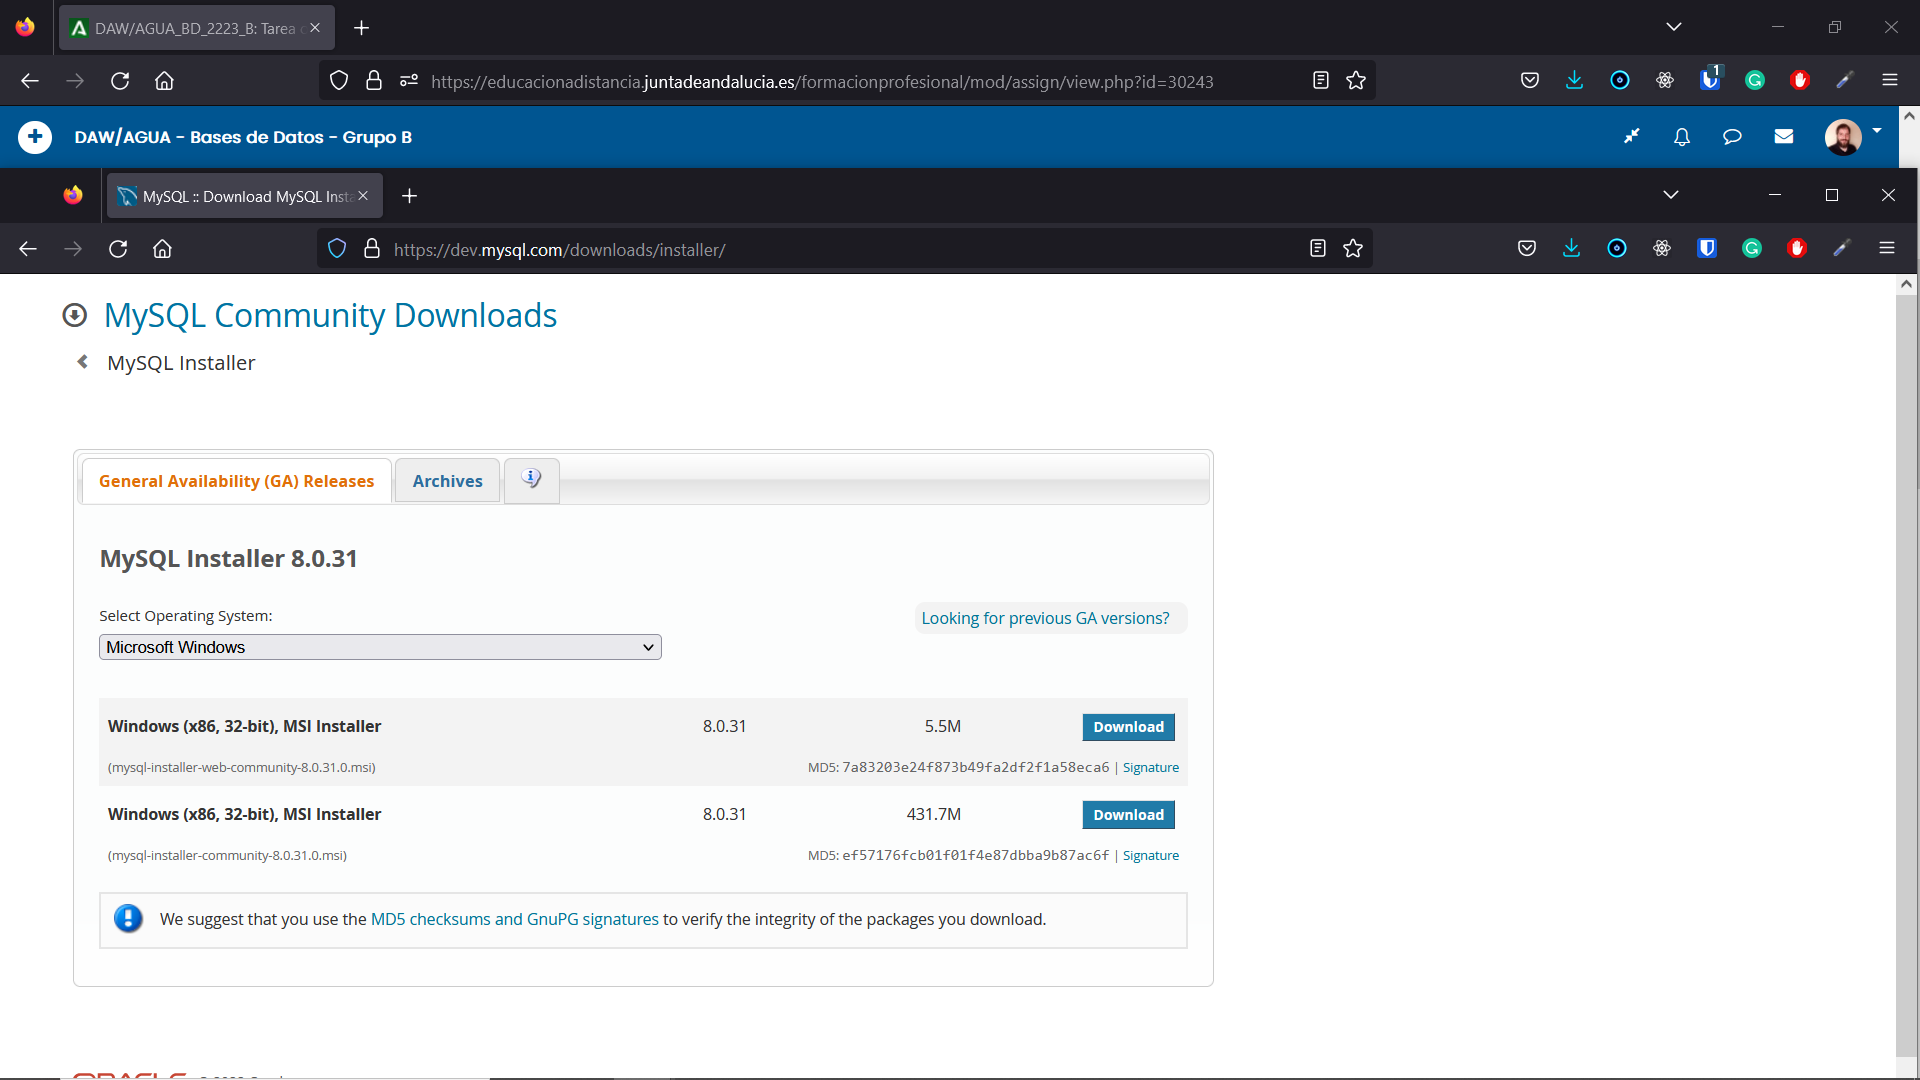
\includegraphics[scale=0.32]{descarga-mysql.png}
        \caption{Página de descarga del instalador de MySQL}
    \end{figure}

    \item \textbf{Instalación}

    Una vez descargado el instalador, lo ejecutamos desde el directorio donde se haya descargado. Esto iniciará el instalador, mostrando una ventana donde nos permitirá elegir que versión de MySQL queremos instalar. Nosotros vamos a elegir la \textbf{Developer Default}, que nos instalará todas las herramientas necesarias para el desarrollo, como podemos ver en la siguiente figura. Una vez seleccionada la opción, pulsaremos en botón ``\textit{Next}''.

   \begin{figure}[ht]
        \centering
        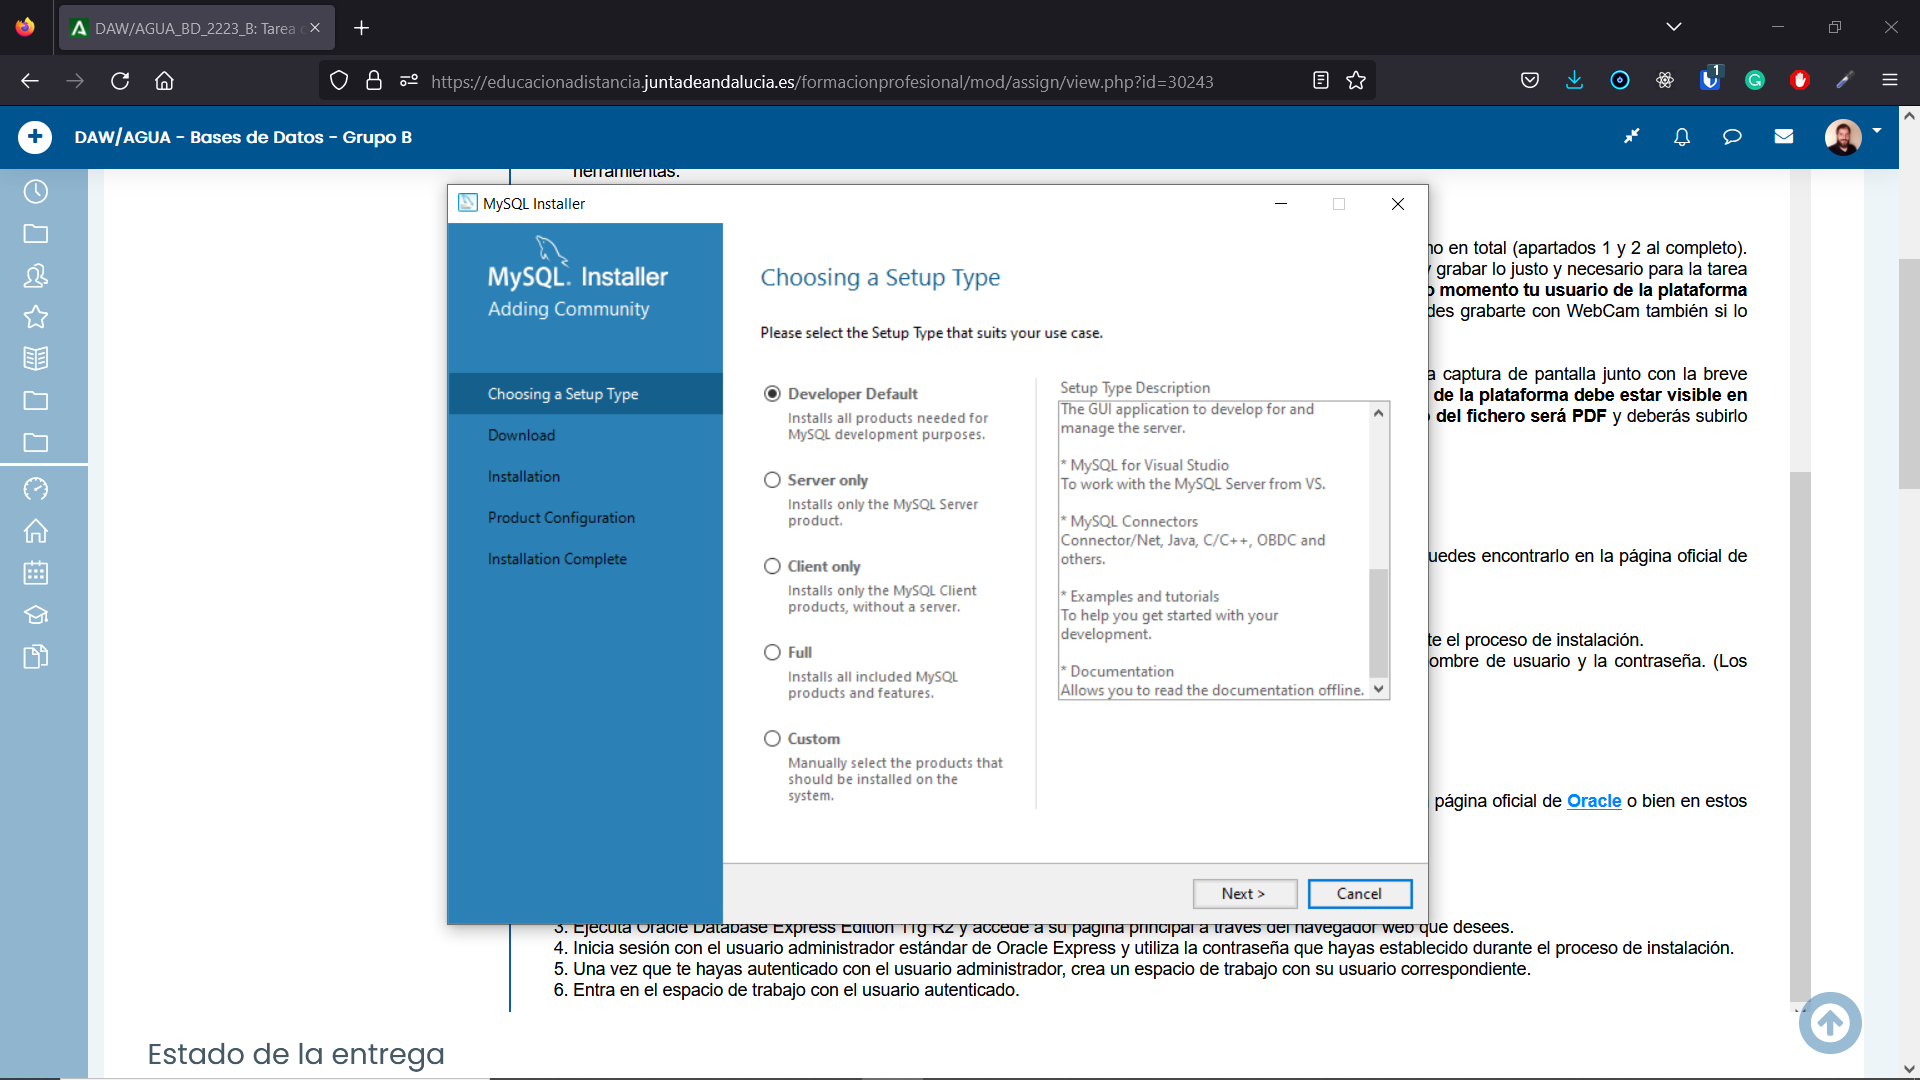
\includegraphics[scale=0.30]{install-mysql-1.png}
        \caption{Pantalla inicial del Instalador de MySQL}
    \end{figure}

    Se nos puede mostrar alguna ventana indicándonos que hay dependencias sin cumplir, por ejemplo, en el caso de que no tengamos instalado el editor Visual Studio. Podemos pulsar en ``\textit{Next}'' sin problema.

    A continuación se nos mostrará una pantalla con todos los componentes que se van a instalar. Pulsamos en ``\textit{Execute}'' y los componentes comenzarán a descargarse y a instalarse, como se puede observar en la siguiente figura.

    \begin{figure}[ht]
        \centering
        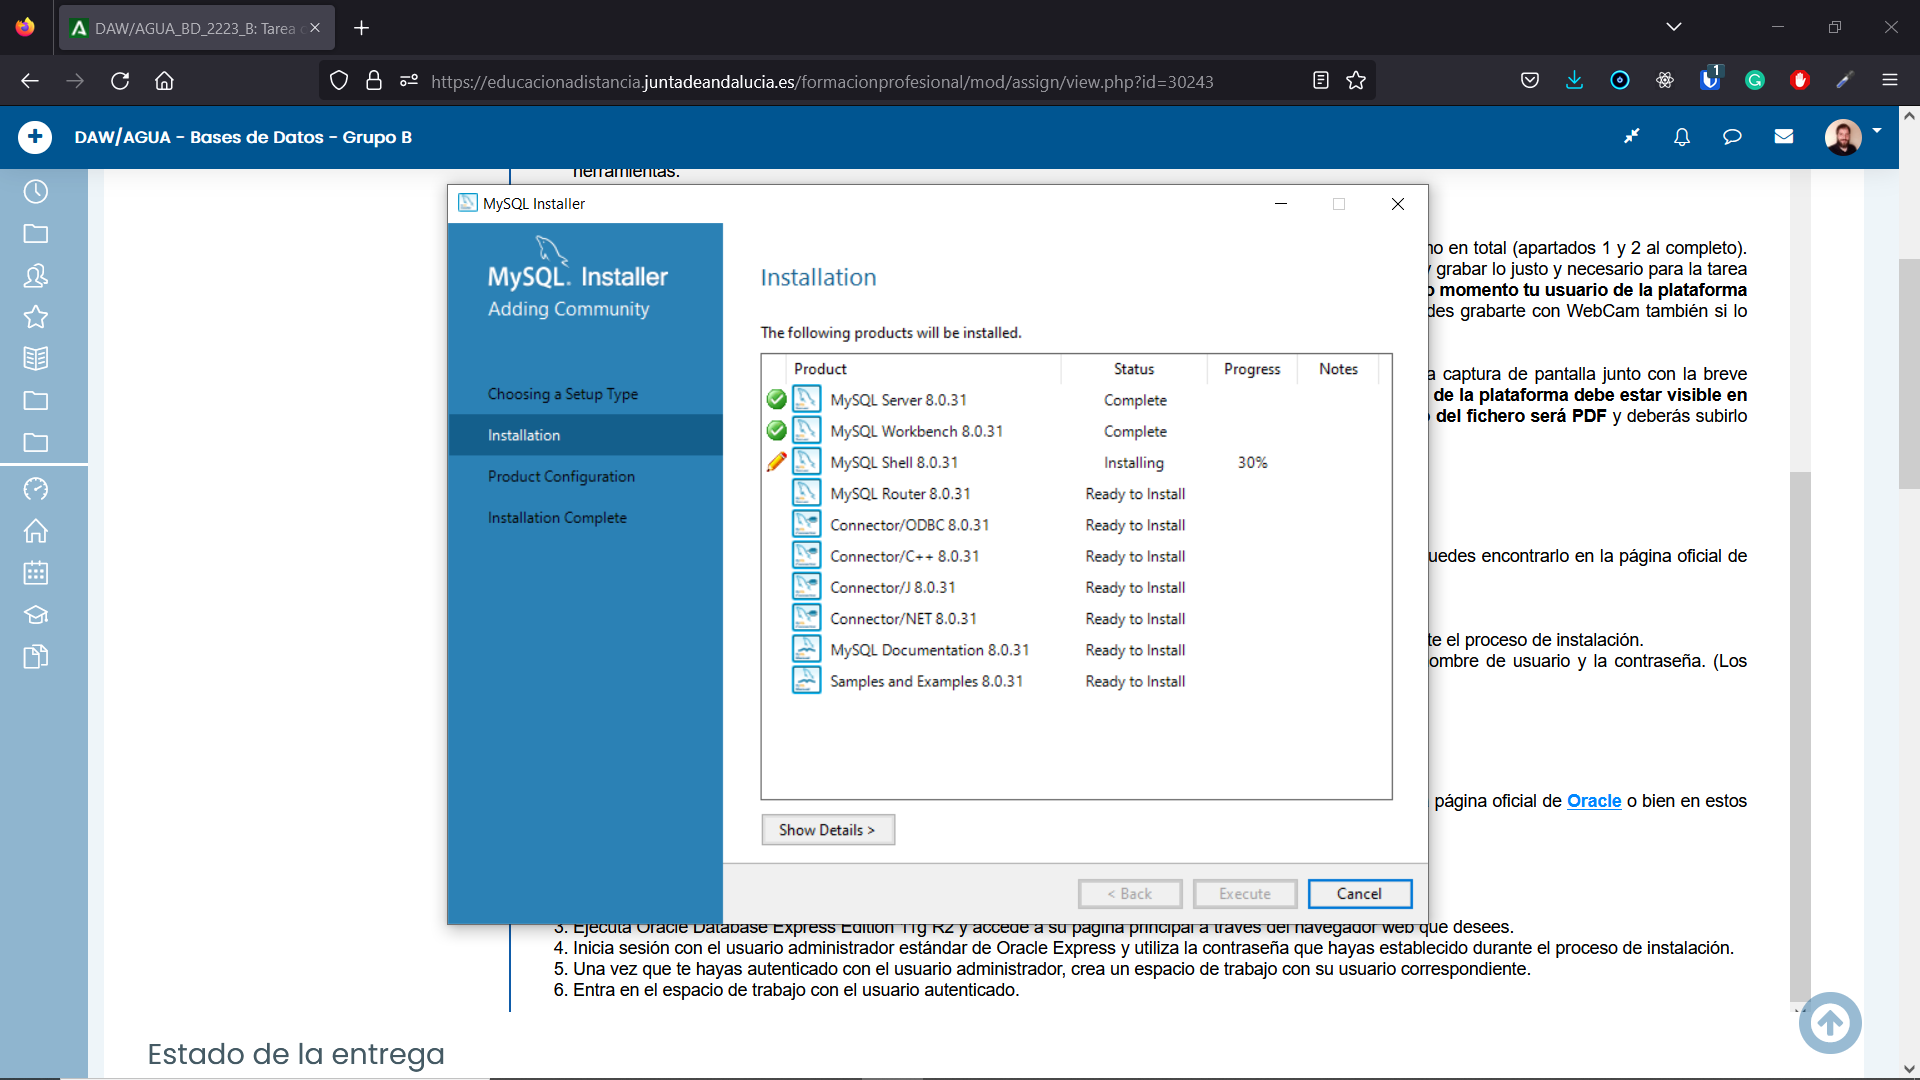
\includegraphics[scale=0.30]{install-mysql-3.png}
        \caption{Descarga e Instalación de componente de MySQL}
    \end{figure}

    Tras la descarga e instalación de componentes, se nos mostrarán diversas pantallas de configuración, aunque como nosotros vamos a seleccionar la configuración por defecto, solo deberemos introducir la \textbf{contraseña de root} en la pantalla que se nos solicite, dejando el resto de datos tal cuál y pulsando en el botón ``\textit{Next}'' hasta que se nos indique que la instalación se ha completado.

    \item \textbf{Ejecución de Workbench y Pantalla Principal}

    Después de realizar la instalación, buscaremos en el menú desplegable de Windows las aplicaciones instaladas. En concreto, vamos a ejecutar \textbf{MySQL Wokbench}, que es la interfaz gráfica oficial de MySQL. Pulsamos en esta aplicación y se nos abrirá la ventana principal. En esta pantalla principal podemos diferenciar los siguientes  elementos:

    \begin{enumerate}[label=\arabic*.]
        \item \textbf{Menu Principal}: contiene diferentes opciones como \textit{file}, \textit{edit}, \textit{view}, etc...
        \item \textbf{Menú Lateral}: donde podemos alternar entre diferentes vistas de la aplicación.
        \item \textbf{Enlaces}: diversos enlaces para acceder a la documentación, los foros o el blog.
        \item \textbf{MySQL Connections}: donde se nos mostrarán las diferentes conexiones que podemos realizar con la base de datos, donde podemos ver que solo tenemos la conexión por defecto creada con el usuario root
    \end{enumerate}

    En la siguiente captura, podemos ver todos estos elementos.

    \begin{figure}[ht]
        \centering
        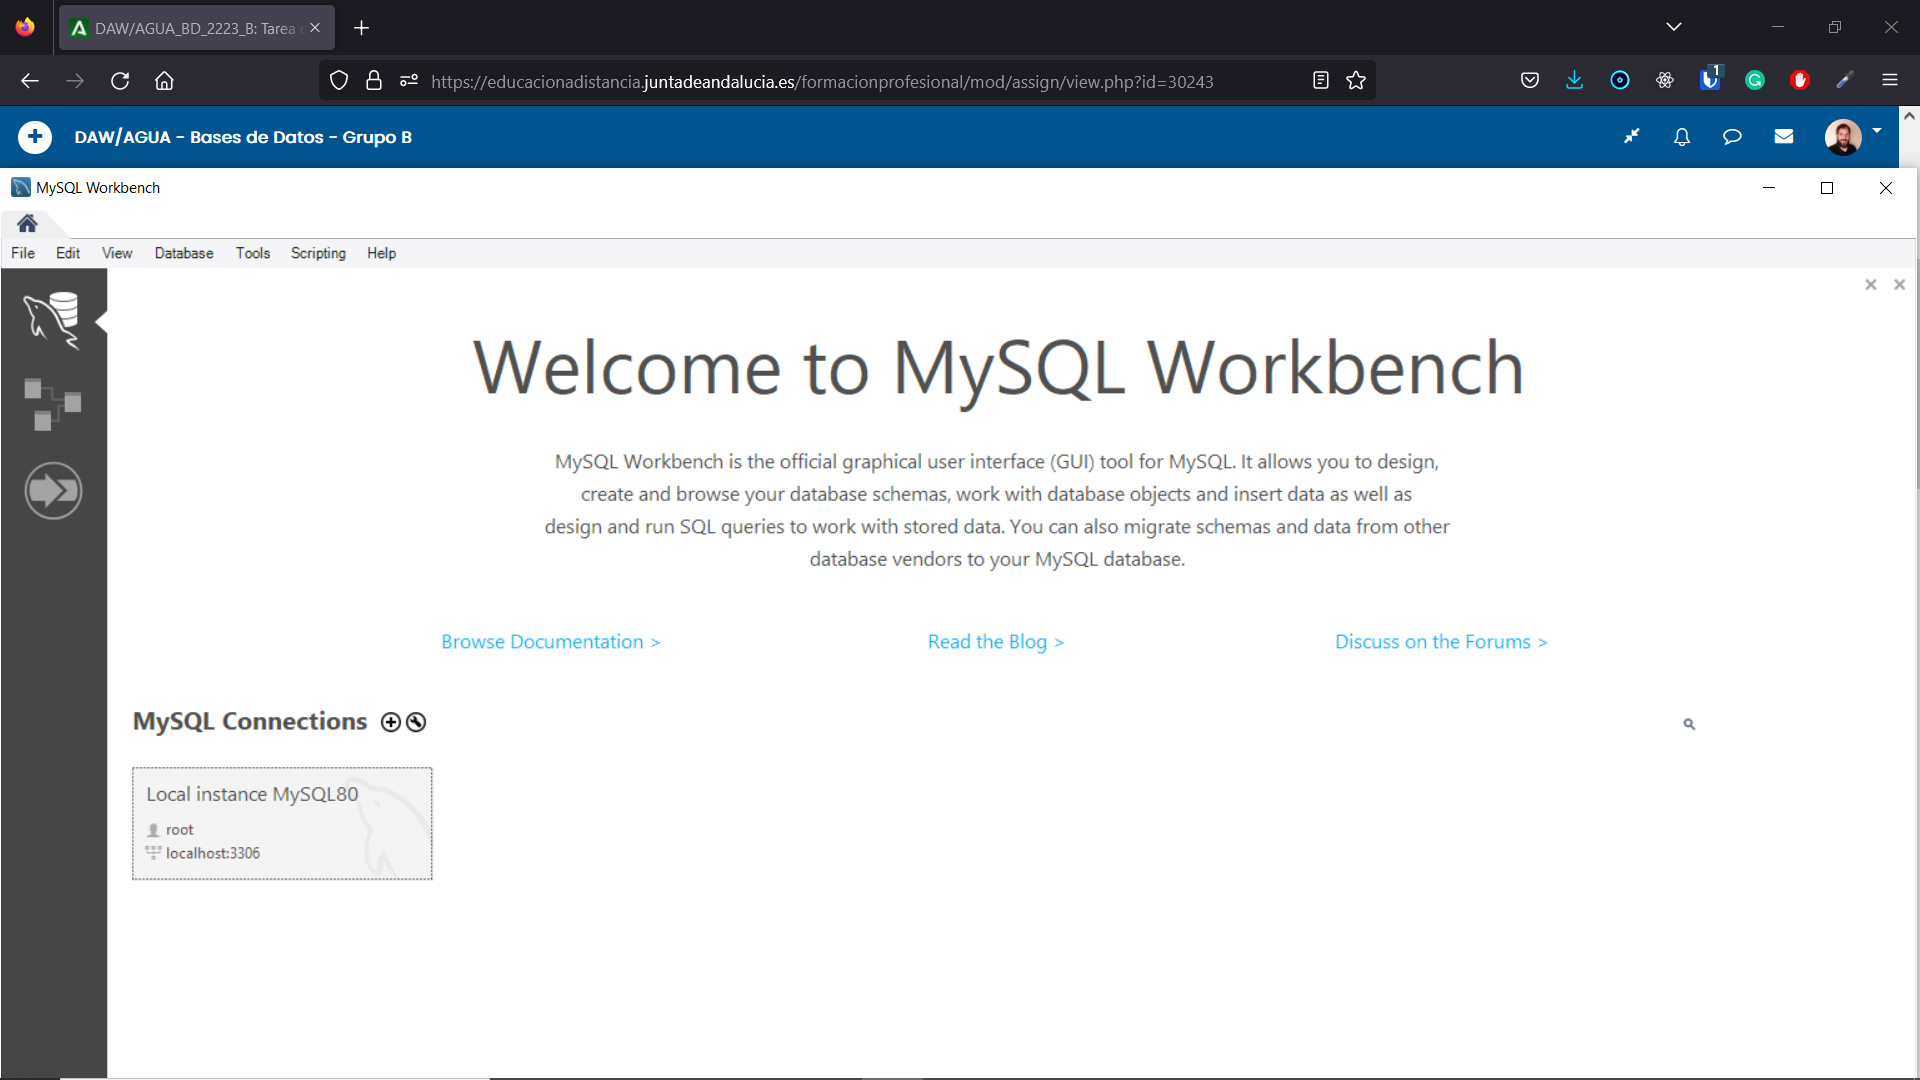
\includegraphics[scale=0.30]{workbench-main.png}
        \caption{Pantalla principal de MySQL Workbench}
    \end{figure}


    \item \textbf{Realizando la Primera Conexión}

    El siguiente paso es realizar una conexión con la base de datos. Ahora mismo solo tenemos la conexión creada durante la instalación para el \textbf{usuario root}, como hemos indicado en el punto anterior. Pulsamos sobre dicha conexión en el apartado \textbf{MySQL Connections} de la pantalla principal y se nos abrirá una ventana pidiéndonos la \textbf{contraseña del usuario root}, que deberíamos haber introducido durante el proceso de instalación.

    Después de haber introducido la contraseña, se realizará la conexión y se nos mostrará la página principal de la conexión, donde se nos permitirá gestionar la base de datos, realizar consultar, etc... Esta pantalla, esta compuesta de los siguientes elementos:

    \begin{enumerate}[label=\arabic*.]
        \item \textbf{Menu Principal y Barra de Herramientas}: en la parte superior nos encontramos el menú principal, con diferentes opciones y desplegables y la barra de herramientas, que nos permite realizar acciones rápidamente, como añadir tablas a la base de datos, filas a una tabla, columnas, etc...
        \item \textbf{Menu Lateral}: este menú nos permite administrar diferentes aspectos de la base de datos, como las conexiones que se han realizado, el número de usuario y sus privilegios, el estado del sistema, etc.., así como consultar diferente información sobre la base de datos como los logs, la performance, etc...
        \item \textbf{Pestaña de Consultas}: en esta pestaña es donde realizare las consultas a la base de datos, usando para ello, principalmente, el lenguaje SQL.
        \item \textbf{Pestaña SQL Additions}: esta pestaña nos permite cargar diferentes herramientas que nos ayudarán a la hora de realizar las consultas, como por ejemplo, snippets para SQL.
        \item \textbf{Pestaña de Salida}: aquí se nos mostrará la salida de las acciones realizadas.
    \end{enumerate}

    \begin{figure}[ht]
        \centering
        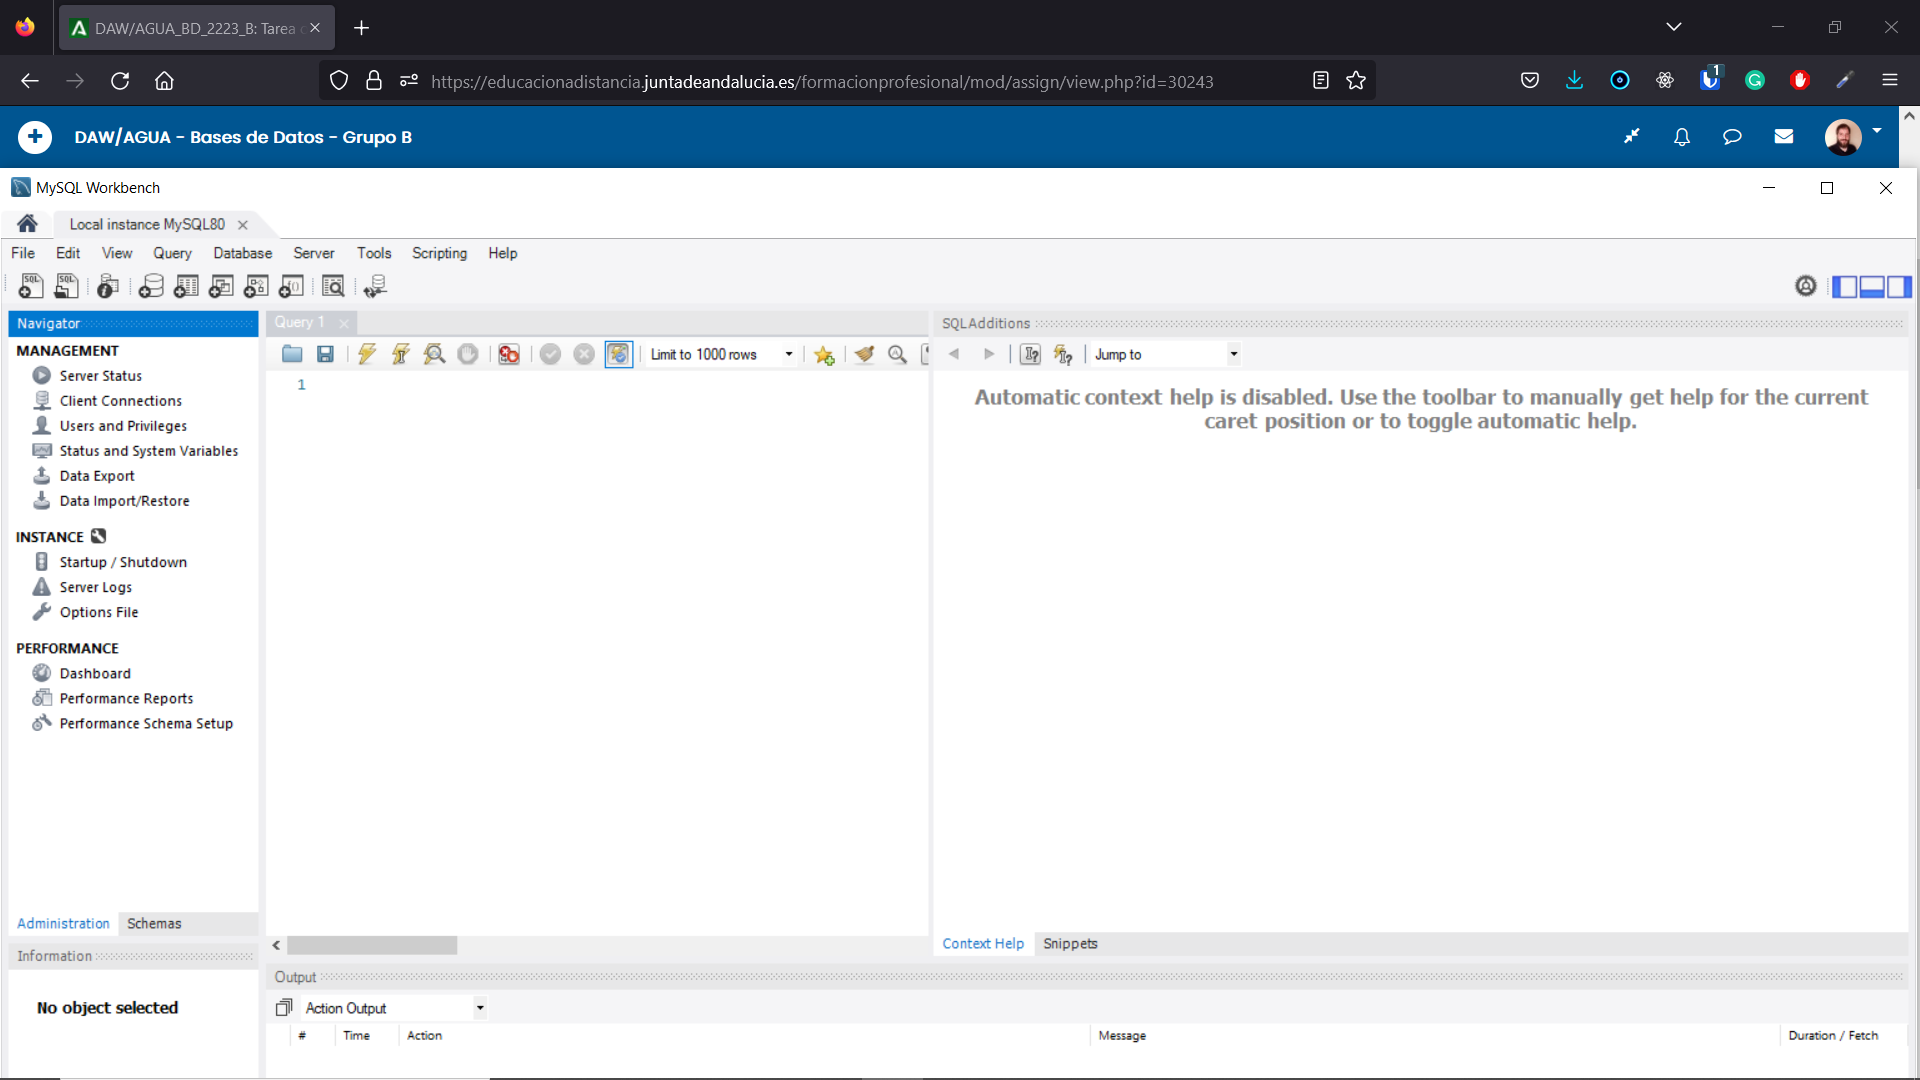
\includegraphics[scale=0.30]{workbench-conection-2.png}
        \caption{Ventana emergente para realizar la conexión con la base de datos}
    \end{figure}

    \item \textbf{Creación de Usuario}

    Ya que tenemos una nueva conexión activa y con privilegios de administrador vamos a crear una nuevo usuario. Para ello, pulsamos en el opción ``\textit{Users and Privileges} del menú lateral en la ventana principal de conexión. Estos nos abrirá una nueva ventana donde se nos mostrará los usuarios que hay ahora mismo creados en la base de datos.

    Pulsamos en la opción ``\textit{Add Account}, que nos encontramos abajo a la izquierda, y se nos abrirá un formulario donde podremos introducir diferentes datos sobre el nuevo usuario. En nuestro caso, solo vamos a cambiar el nombre de usuario a \textbf{fcosueza} y a introducir \textbf{una contraseña}. Debemos introducir una contraseña que nos sea fácil de recordar, aunque hay que tener en cuenta en en entornos de producción esto sería un error muy grande, ya que las contraseña tienen que ser suficientemente fuertes y complejas para no comprometer la seguridad de la base de datos.

    Una vez que hayamos introducido la información, pulsamos en el botón ``\textit{Apply} y nuestro usuario se habrá creado. En la siguiente figura podemos ver una captura de la pestaña de creación de usuarios.

    \newpage

    \begin{figure}[ht]
        \centering
        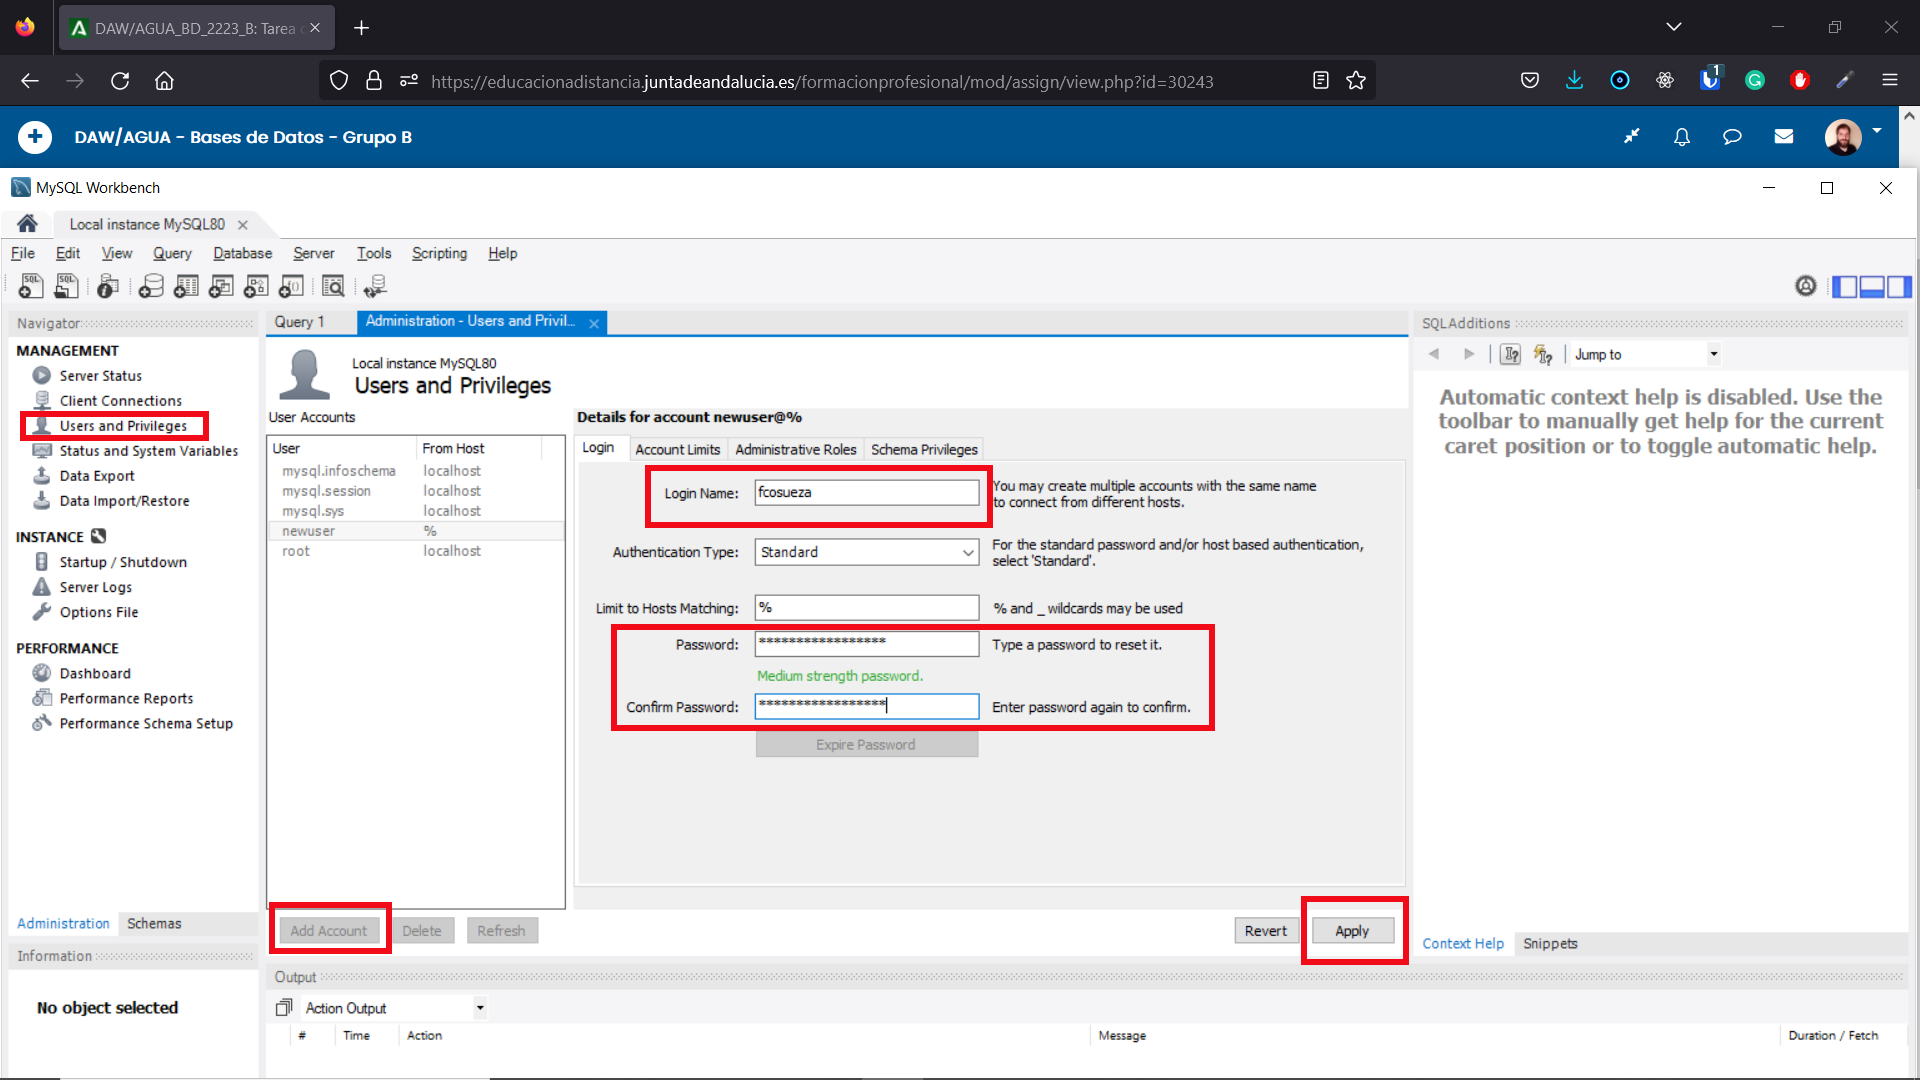
\includegraphics[scale=0.30]{create-user.png}
        \caption{Sección de Empleo Público del IAAP}
        \label{fig:create}
    \end{figure}

    \item \textbf{Conexión con el Nuevo Usuario}

    Una vez creado el usuario, ya solo nos queda realizar una conexión a la base de datos con éste.
\end{enumerate}




% Bibliography

\newpage
\bibliography{citas}
\bibliographystyle{unsrt}

\end{document}